\section{Введение}
\subsection{Теоритическая часть}

\textbf{Цель работы:}
исследование вынужденных колебаний и процессов их уста­новления в колебательном контуре.

\textbf{В работе используются:}
генератор звуковых частот, вольтметр, часто­томер, конденсатор, катушка индуктивности, магазин сопротивлений, ос­ циллограф, универсальный измеритель импеданса ($LCR$-метр).

\begin{wrapfigure}[14]{r}{0.4\linewidth}
	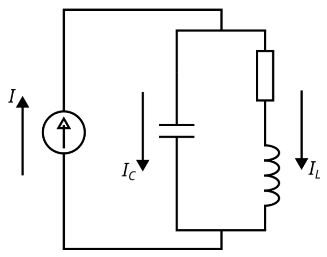
\includegraphics[width=\linewidth]{shem.png}
	\caption{Описываемый RLC контур}
\end{wrapfigure}
\noindent Для RLC контура (рис. 1) применим 2 правило Кирхгофа:
\begin{equation}
    RI + U_C + L\frac{dI}{dt} = 0.
\end{equation}
Подставив в уравнение (1) выражение для тока через 1-ое правило Кирхгофа, и разделив обе части уравнения на $CL$, получим:
\begin{equation}
    \frac{d^2U_C}{dt^2} + \frac{R}{L} \frac{dU_C}{dt} + \frac{U_C}{CL}.
\end{equation}
Произведём замены $\gamma = \frac{R}{2L}$ -- коэффициент затухания, $\omega_0^2 = \frac{1}{LC}$ -- собственная круговая частота, $T_0 = \frac{2\pi}{\omega_0} = 2\pi \sqrt{LC}$ -- период собственных колебаний. Тогда уравнение (2) примет вид:
\begin{equation}
    \ddot{U_C} + 2 \gamma \dot{U_C} + \omega_0^2U_C = 0,
\end{equation}
где точкой обозначено дифференцирование по времени. Будем искать решение данного дифференциального уравнения в классе функций следующего вида:
$$U_C(t) = U(t)e^{- \gamma t}.$$
Получим:
\begin{equation}
    \ddot{U} + \omega_1^2 U = 0,
\end{equation}
где
\begin{equation}
    \omega_1^2 = \omega_0^2-\gamma^2
\end{equation}
Для случая $\gamma < \omega_0$ в силу того, что $\omega_1 > 0$, получим:
\begin{equation}
    U_C(t) = U_0 \cdot e^{-\gamma t} \text{cos}(\omega_1 t + \varphi_0).
\end{equation}
Для получения фазовой траектории представим формулу (6) в другом виде:
\begin{equation}
    U_C(t) = e^{-\gamma t}(a \text{cos} \omega_1 t + b \text{sin} \omega_1 t),
\end{equation}
где $a$ и $b$ получаются по формулам:
$$a = U_0 \text{cos} \varphi_0, \qquad b = - U_0 \text{sin} \varphi_0.$$
В более удобном виде запишем выражения для напряжения на конденсаторе и токе через катушку:
\begin{equation}
    U_C (t) = U_{C0} \cdot e^{-\gamma t} (\text{cos} \omega_1 t + \frac{\gamma}{\omega_1} \text{sin} \omega_1 t),
\end{equation}
\begin{equation}
    I(t) = C\dot{U_C}= - \frac{U_{C0}}{\rho} \frac{\omega_0}{\omega_1} e^{-\gamma t} \text{sin} \omega_1 t.
\end{equation}
Введём некоторые характеристики колебательного движения:
\begin{equation}
    \tau = \frac{1}{\gamma} = \frac{2L}{R},
\end{equation}
где $\tau$ -- время затухания (время, за которое амплитуда колебаний уменьшается в $e$ раз).
\begin{equation}
    \Theta = \text{ln} \frac{U_k}{U_{k+1}} = \gamma T_1 = \frac{1}{N_\tau} = \frac{1}{n} \text{ln} \frac{U_k}{U_{k+n}},
\end{equation}
где $\Theta$ -- логарифмический декремент затухания, $U_k$ и $U_{k+1}$ -- два последовательных максимальных отклонения величины в одну сторону, $N_\tau$ -- число полных колебаний за время затухания $\tau$.

Теперь рассмотрим случай \textit{вынужденных колебаний} под действием внешней внешнего синусоидального источника. Для этого воспользуемся методом \textit{комплексных амплитуд} для схемы на рисунке (рис. 1):
\begin{equation}
    \ddot{I} + 2 \gamma \dot{I} + \omega^2 I = - \varepsilon \frac{\Omega}{L} e^{i\Omega t}.
\end{equation}
Решая данное дифференциальное уравнение получим решение:
\begin{equation}
    I = B\cdot e^{-\gamma t} \text{sin}(\omega t - \Theta) + \frac{\varepsilon_0 \Omega}{L \phi_0} \text{sin} (\Omega t - \varphi).
\end{equation}
Нетрудно видеть, что частота резонанса будет определяться формулой:
\begin{equation}
    \omega_0 = \frac{1}{2 \pi \sqrt{LC}}.
\end{equation}

Способы измерения \textbf{добротности}:
\begin{enumerate}
    \item с помощью потери амплитуды свободных колебаний:
    \begin{equation}
        Q = \frac{1}{n} \text{ln}\frac{U_k}{U_{k+n}},
    \end{equation}
    \item с помощью амплитуды резонанса можно получить добротность (в координатах $U_C/U_0$, где $U_0$ -- амплитуда колебаний напряжения источника, от частоты генератора). Отсюда нетрудно определить декремент затухания $\gamma = \frac{\omega_0}{2Q}$,
    \item с помощью среза АЧХ на уровне 0.7 от максимальной амплитуды, тогда <<дисперсия>> ($\Delta \Omega$) будет численно равна коэффициенту $\gamma$, то есть $Q = \frac{\nu_0}{2 \Delta \Omega}$.
    \item с помощью нарастания амплитуд в вынужденных колебаниях:
    \begin{equation}
        Q = \frac{\omega_0 n}{2\text{ln} \frac{U_0 - U_k}{U_0 - U_{k+n}}}.
    \end{equation}
\end{enumerate}

\subsection{Экспериментальная установка}
Схема установки для изучения собственных колебаний представлена на рисунке (2), по ходу работы она будет претерпевать некоторые изменения, связанные со съёмом сигнала с различных её частей, что на принцип работы не повлияет, основным же изменением будет смена работы генератора сигналов, соответствующий режим будет описан в практической части, при переходе на него. Пунктиром показана схема подключения при снятия данных о колебаниях в фазовой плоскости, на рисунке (3) изображена схема установки для исследования АЧХ, ФЧХ и наблюдения биений.

\begin{figure}[h]
    \centering
    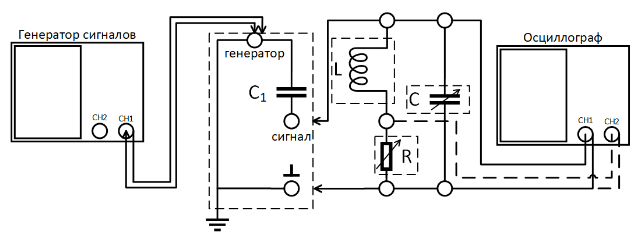
\includegraphics[width=0.8\linewidth]{ustan1.png}
    \caption{Схема установки для изучения собственных колебаний}
\end{figure}

\begin{figure}[h]
    \centering
    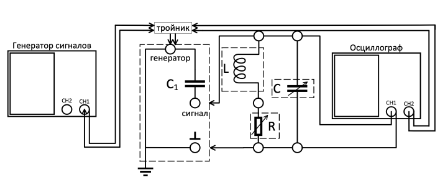
\includegraphics[width=0.8\linewidth]{ustan2.png}
    \caption{Схема установки для изучения вынужденных колебаний и биений}
\end{figure}

Красным прямоугольником выделен колебательный контур, \textit{<<состояния>>} элементов так же будут описаны в практической части. Конденсатор ($C_1$) между генератором сигналов и колебательным контуром служит для того, чтобы импеданс генератора был много меньше импеданса колебательного контура и не влиял на процессы, происходящие в контуре.
